\documentclass[11pt,a4paper]{article}
\usepackage[margin=2.4cm]{geometry}
\usepackage{booktabs,tabularx,graphicx,enumitem}
\usepackage[hidelinks]{hyperref}
\usepackage{parskip}
\setlist{itemsep=2pt,topsep=3pt}
\emergencystretch=2em
\graphicspath{{../oracle_audit/paper/}}

\title{Project report: from drift detection to the validity of RAG tests}
\author{Aditi Saxena, Suvidh Jain and Aryan Garg}
\date{18 October 2026}

\begin{document}
\maketitle

\section*{Summary}
This report describes how the project developed and where it stands now. We began with label-free
drift detection for retrieval-augmented generation (RAG) systems. An audit of that work showed that
the detectors could not see the most common harmful change, an edited fact, and the remaining
questions in that area turned out to be largely answered in the literature. Two further ideas did
not pass the tests we had set for them in advance.

We then turned to a metamorphic-testing framework for RAG published at ASE~2026 by Kim, Pasini and
Tonella. Its counterfactual test adds a passage that contradicts a fact in the documents and checks
whether the system's answer changes. In its released code, any change in the answer counts as a pass,
and the answer is not compared with the injected fact. In the authors' released outputs, at least
77\% of the reported counterfactual faults are answers that match the dataset's ground truth, and
26\% of the counterfactual inputs are refusals written by the model that was asked to generate them.
We proposed an alternative test and evaluated it with three small open models.

The results are written up as a draft journal manuscript. It has not been submitted. Two steps are
still outstanding: a human check of our automatic scoring, and contacting the original authors.

\section{How the project started}
The project began as \emph{Drift-Aware RAG}, based on a working paper from July 2026. The idea was to
monitor the embeddings of a RAG system's documents and queries and to raise an alarm when their
distribution shifted, without needing labelled answers. Aryan wrote the base pipeline. Aditi owned
the repository and ran the first analysis. Suvidh then carried out an independent audit and a set of
validation experiments, recorded in \texttt{quarantine/FINDINGS.md} (dated 5 September 2026).

The audit found that the pipeline as first written could not produce valid numbers, and it was
rebuilt. Two planned experiments passed: drift thresholds calibrated by permutation held across query
volumes, and a probe-based selective re-index saved embedding compute at a small cost in recall. A
third, unplanned result changed the direction of the project. When documents were edited in place,
retrieval lost about 30 points of recall@10, while the drift statistic stayed at the level of noise.
In other words, the detector could monitor changes in the queries but could not see stale documents.
A literature review in early October also showed that label-free drift detection is well served by
existing tools, and that estimating accuracy without labels is impossible in general. We kept these
results as a negative finding.

\section{How the direction changed}
Table~\ref{tab:timeline} summarises the sequence. The literature shaped several of the decisions.
HoH (ACL~2025) and a 2026 study of stale-document poisoning had already shown that outdated evidence
harms RAG answers and that models make limited use of dates, so measuring answer-level staleness on
its own would not have been new. Work on how models should answer when sources conflict (DRAGged into
Conflicts, 2025; WikiContradict, 2024) gave us a reference for good behaviour. The question we
eventually asked, whether injected faults stand for real ones, has a long history in software
testing, for example in Just et al.\ (FSE~2014).

\begin{table}[h]
\centering
\small
\caption{Timeline of the project.}
\label{tab:timeline}
\begin{tabularx}{\linewidth}{@{}l X X@{}}
\toprule
When & What was done & Outcome \\
\midrule
Until Sep 2026 & Base pipeline (Aryan); independent audit, validation experiments and rebuild (Suvidh) & Detectors work for query-side change but cannot see edited facts \\
9--10 Oct & Answer-level staleness. Two pre-registered ideas tested: scheduling re-fetches by how often facts change, and keeping old embeddings while refreshing the text & Both failed their pre-set criteria; the underlying harm was already documented \\
10--13 Oct & Tests with real Wikipedia revisions, intended to extend the ASE~2026 framework & Early results were encouraging; one large run was void twice and had to be redesigned \\
13 Oct & A critical review of our own results & The ``real revisions'' idea overlapped with HoH, and one comparison had been mapped the wrong way round; both corrected \\
13--16 Oct & Reading of the ASE~2026 code and released outputs & The counterfactual test does not compare answers with the injected fact; this became the subject of the manuscript \\
13--17 Oct & Pre-registered experiments with an alternative test & Results in Section~\ref{sec:results} \\
\bottomrule
\end{tabularx}
\end{table}

\section{What we found}
\label{sec:results}

\subsection*{The published counterfactual test}
The ASE paper states that, after a counterfactual fact is injected, the answer should ``align with
the injected fact''. In the released code, the verdict depends only on whether the answer changed.
As a result, a system that keeps the original, correct answer is counted as faulty, any changed answer
passes, and a fault is recorded as repaired whenever the new answer differs from the original correct
one. The paper also describes the expected behaviour in more than one way: in some places it asks
the system to signal the conflict, in others to adopt the new fact.

Using the authors' released outputs, we first reproduced their main table in all ten cells. Of the 594
counterfactual faults reported in the paper, at least 460 (77\%) are answers that match the dataset's
ground truth. Of the 2,671 counterfactual inputs, 694 (26\%) are refusals such as ``Sorry, I can't
help create misleading counterfactuals\ldots''. The share is highest in one setting, at 48\%
(Figure~\ref{fig:refusals}). In one of the paper's own examples, a case described as a fault that
``persisted after repair'' is recorded in the released outputs as repaired.

Two of our pre-registered expectations about their data were not confirmed. Where the counterfactual
was placed in the document made no measurable difference, and most answers that passed did follow the
injected value. These findings concern the released code and data at one version; the authors may
have intended a different reading of the test, which is one reason we want to hear from them before
submitting.

\begin{figure}[h]
\centering
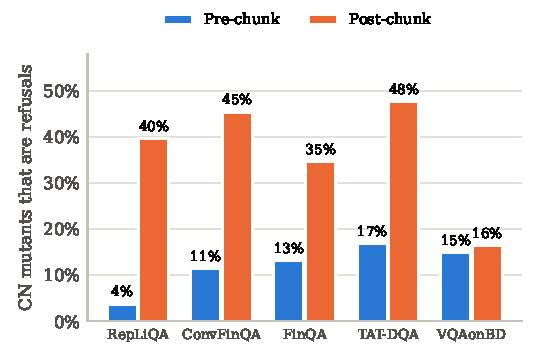
\includegraphics[width=0.58\linewidth]{fig_refusals.pdf}
\caption{Share of the ASE counterfactual inputs that are refusals, per dataset and mode.}
\label{fig:refusals}
\end{figure}

\subsection*{An alternative test}
Our alternative gives each of the two conflicting values a date and then swaps only the dates. A
system that follows the dates should change its answer when they are swapped, so the expected answer
follows from the input and no answer key is needed. We built 392 questions from real Wikipedia
updates and ran three open models locally. For the two smaller models, the published test reports
fewer date-related failures than the date-swap test finds: 8\% against 41\% for Qwen-7B and 30\%
against 51\% for phi3 (Figure~\ref{fig:rates}). The two tests mostly flag different questions.

The results for the largest model, Qwen-14B, were less clear. It usually listed both values instead of
choosing one, which neither test counts as a fault. A follow-up showed that our prompt was largely
responsible for this. When asked for a single answer, the model followed the newer date in 59\% of
cases, just below the 60\% we had set in advance for calling it date-following, so we report the
result as mixed. The alternative test also has limits: it assumes the newest value should win, and it
relies on dates written in the text.

\begin{figure}[h]
\centering
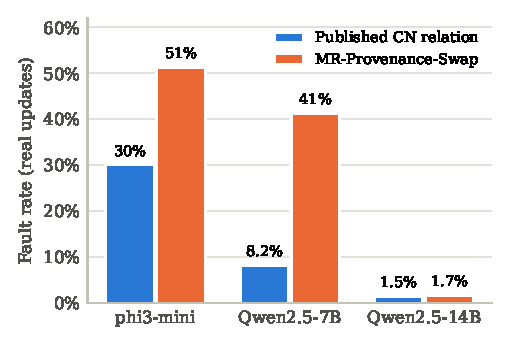
\includegraphics[width=0.52\linewidth]{fig_rates.pdf}
\caption{Fault rates on real updates under the published test and under the date-swap test.}
\label{fig:rates}
\end{figure}

\section{What did not work, and what we corrected}
One pre-registered prediction failed: the two tests disagree about which cases are faulty for the two
smaller models, but not for the largest one. A pilot comparing two answering strategies did not pass
its pre-set gate, so the full experiment was not run. One large data run was void twice before it was
redesigned. We also corrected several of our own mistakes. The refusal rate was first counted as
12.5\% and rose to 26\% after we found a bug in the detection pattern. One earlier comparison had been
mapped the wrong way round. We withdrew a claim about the order of passages after it did not survive
checking. All of these are recorded in the project's claims register.

\section{How the work was done}
Hypotheses and pass/fail thresholds were written down and the analysis scripts were fingerprinted
before each main run. All models ran locally through Ollama; no paid services were used. A script
checks every citation and quotation in the manuscript against the original sources. Much of the work
in October, including writing and running the analysis scripts, searching the literature and drafting
documents, was done with the help of an AI assistant (Claude Code). We checked its output against the
data and logs, and the manuscript declares this use, as both Elsevier and IEEE require.

\section{Current state}
The manuscript is a draft, prepared in Elsevier format (22 pages) and IEEE format (9 pages). Before it
can be submitted:
\begin{itemize}
  \item Suvidh and Aryan need to label 200 cases independently, so that our automatic scoring can be
        compared with human judgement.
  \item We need to send our findings to the ASE authors and allow them time to respond.
  \item We need to add affiliations, agree the author contributions, and review the AI-use statement.
\end{itemize}
The main limitations are that our experiments use three small open models and one domain (Wikipedia
infobox values), and that the audit covers one framework.

\section{Questions for you}
\begin{enumerate}
  \item Is a paper about the validity of a published test a suitable submission for a
        software-testing journal such as JSS or IST, or an IEEE journal?
  \item Should we contact the ASE authors before submitting, as we plan to?
  \item Is an audit of one framework, together with general criteria and an alternative test, enough
        scope, or should we examine a second framework?
  \item Would the negative results on drift detection be worth a separate short paper?
\end{enumerate}

\end{document}
